\documentclass[10pt,a4paper,twocolumn]{article}

\usepackage[spanish]{babel}
\usepackage[utf8]{inputenc}
\usepackage[T1]{fontenc}
\usepackage{graphicx}
\usepackage{booktabs}
\usepackage{geometry}
\usepackage{hyperref}
\usepackage{microtype}

\geometry{left=1.6cm,right=1.6cm,top=1.8cm,bottom=1.8cm}
\setlength{\columnsep}{0.65cm}

\title{\textbf{Sistema de vision artificial para el control de un sumobot con ESP32-CAM}}
\author{Juan Jose Prado Neira}
\date{Junio de 2026}

\begin{document}
\maketitle

\begin{abstract}
Este articulo presenta un prototipo de vision artificial para controlar un
robot tipo sumobot mediante una arquitectura distribuida. Una ESP32-CAM envia
video por UDP a un portatil, donde OpenCV procesa la imagen, detecta las lineas
del carril y localiza objetos que invaden la trayectoria. A partir de esta
informacion se genera una accion de alto nivel que se envia por UDP a un segundo
controlador encargado de los motores. El sistema combina seguimiento reactivo
de carril, control manual y una rutina de expulsion de objetos formada por
aproximacion, empuje y reincorporacion marcha atras. Las pruebas internas
registradas suman 18.891 frames y 677,70 s, con una frecuencia media aproximada
de 27,88 FPS.
\end{abstract}

\noindent\textbf{Palabras clave---} vision artificial, OpenCV, ESP32-CAM,
robotica movil, UDP, sumobot.

\section{Introduccion}

La robotica movil de bajo coste permite construir demostradores completos de
percepcion, decision y actuacion con recursos reducidos. En este trabajo se
aborda el control de un sumobot que debe navegar entre dos lineas y retirar
objetos situados en su trayectoria. El objetivo principal no es entrenar un
modelo generalista, sino obtener una cadena funcional y ajustable para una
demostracion docente: capturar imagen, procesarla en tiempo real, decidir una
maniobra y ejecutar la orden sobre el robot.

El sistema aprovecha una arquitectura distribuida. La camara y los motores se
mantienen en placas ESP32, mientras que el portatil concentra el procesamiento
visual y la depuracion. Esta separacion reduce la carga embarcada, facilita el
ajuste de parametros y permite visualizar en directo las mascaras y decisiones
que produce el algoritmo.

\section{Metodologia}

La solucion se implementa como una cadena de cuatro bloques. El primer bloque
recibe frames JPEG fragmentados por UDP y reconstruye una imagen BGR de OpenCV.
El segundo bloque procesa cada frame: redimensiona la imagen, aplica una region
de interes inferior, opcionalmente transforma la perspectiva y construye una
mascara de lineas oscuras mediante contraste local, umbral absoluto y
morfologia. A partir de los contornos calcula candidatos de linea izquierda y
derecha y estima el centro del carril.

El detector de objetos trabaja en paralelo sobre regiones oscuras de baja
saturacion. Los objetos detectados se devuelven como entidades con posicion,
tamano, area, relacion de aspecto y contador de fusion. Si dos detecciones se
encuentran apiladas o muy proximas verticalmente, se fusionan para evitar que
el robot trate un mismo obstaculo como varios. Ademas, la zona del objeto se
elimina de la mascara de linea para reducir falsos positivos cuando el objeto
se confunde con una marca del carril.

El tercer bloque toma la decision. En seguimiento normal combina offset lateral,
confianza y una regulacion proporcional--integral--derivativa sencilla para
generar avance o curva. Cuando el objeto cumple umbrales de area, posicion
frontal y centrado, se activa un protocolo con estados: enfoque, aproximacion,
empuje lateral y reincorporacion marcha atras. El cuarto bloque traduce la
accion a comandos UDP ASCII para el firmware de motores, incluyendo avance,
curvas suaves, marcha atras y parada segura.

\section{Arquitectura del sistema}

\begin{figure}[t]
\centering
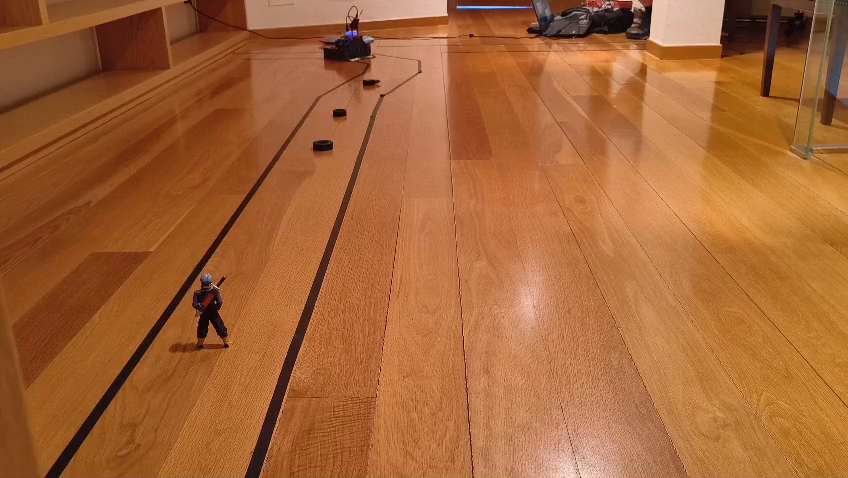
\includegraphics[width=\linewidth]{figures/demo_frame.png}
\caption{Vista de demostracion del sistema durante una ejecucion registrada.}
\label{fig:demo}
\end{figure}

El punto de entrada es \texttt{main.py}, que carga dinamicamente los bloques y
sus ficheros \texttt{config.json}. La ESP32-CAM envia video al portatil en
\texttt{0.0.0.0:5005}. El robot de motores recibe comandos UDP en la direccion
configurada en el bloque de envio. La interfaz de ejecucion muestra cuatro
paneles: camara con decision, mascara, ROI detectada y vista bird/debug.

La configuracion se separa por responsabilidades. El bloque de recepcion define
puerto, timeout y rotacion; el de vision controla umbrales, ROI, perspectiva y
deteccion de objetos; el de decision fija ganancias, tiempos y protocolo de
expulsion; el de envio define IP, puerto y velocidades nominales.

\section{Resultados}

Las pruebas internas se analizaron a partir de los CSV generados por el
registrador de depuracion. No constituyen un benchmark formal, pero permiten
comprobar la estabilidad temporal del prototipo y la distribucion de decisiones
en sesiones reales.

\begin{table}[h]
\centering
\caption{Resumen de ejecuciones registradas.}
\label{tab:resultados}
\begin{tabular}{lrrrr}
\toprule
Sesion & Frames & Tiempo (s) & FPS & Conf. \\
\midrule
13:04 & 1.518 & 54,74 & 27,73 & 0,579 \\
13:04b & 2.407 & 87,06 & 27,65 & 0,526 \\
13:06 & 2.993 & 107,50 & 27,84 & 0,765 \\
13:08 & 11.973 & 428,40 & 27,95 & 0,803 \\
\midrule
Total & 18.891 & 677,70 & 27,88 & 0,744 \\
\bottomrule
\end{tabular}
\end{table}

En el total de frames, el sistema detecto dos lineas en el 65,3\% de los casos,
una sola linea izquierda en el 15,4\%, una sola linea derecha en el 7,5\% y
perdida de lineas en el 11,4\%. La confianza media fue de 0,744 y el offset
absoluto medio registrado fue de 48,7 pixeles. En cuanto a las ordenes enviadas
cuando el movimiento estaba activo, las mas frecuentes fueron avance
(23,3\%), curva izquierda (13,0\%), marcha atras curva izquierda (6,6\%) y curva
derecha (4,1\%). La presencia de muchos frames sin envio se debe al bloqueo de
movimiento o al antirrebote temporal del emisor.

\section{Discusion}

El prototipo consigue integrar comunicacion, percepcion y control en tiempo
real con hardware economico. La frecuencia registrada, cercana a 28 FPS, es
suficiente para una demostracion de laboratorio. La principal ventaja del
enfoque clasico con OpenCV es su interpretabilidad: cada mascara y contorno se
puede visualizar y ajustar durante la prueba. Como contrapartida, el rendimiento
depende de la iluminacion, del contraste de las lineas y de la apariencia de los
objetos.

La rutina de expulsion resuelve el caso practico planteado: detectar un objeto,
empujarlo lateralmente y volver hacia atras con una curva coherente con el
sentido de empuje. Las limitaciones principales son la falta de odometria, la
ausencia de una medida fisica de distancia al objeto y el uso de tiempos fijos
para las fases de maniobra.

\section{Conclusiones}

Se ha desarrollado un sistema funcional de vision y control para un sumobot
basado en ESP32-CAM y OpenCV. El programa recibe video por UDP, detecta carril
y objetos, decide acciones en modo automatico o manual y envia comandos al
robot. La documentacion Sphinx y la estructura por bloques facilitan la entrega
y mantenimiento del proyecto. Como trabajo futuro se propone incorporar
odometria, medir latencia extremo a extremo y sustituir parte de los umbrales
por modelos de segmentacion entrenados con datos propios.

\begin{thebibliography}{9}
\bibitem{opencv}
G. Bradski, ``The OpenCV Library,'' \emph{Dr. Dobb's Journal of Software
Tools}, 2000.

\bibitem{esp32}
Espressif Systems, ``ESP32 Series Datasheet,'' 2024.

\bibitem{vision}
R. Szeliski, \emph{Computer Vision: Algorithms and Applications}. Springer,
2022.
\end{thebibliography}

\end{document}
